\chapter{АНАЛІЗ МЕТОДОЛОГІЧНИХ ОСНОВ РОЗРОБКИ ЗАСОБІВ КІБЕРНЕТИЧНОГО ВПЛИВУ }
\label{1section::doc}\label{1section:id1}

%TODO на початку вказати на необхідність організації КА

\section{Організація, принципи розробки засобів кібернетичного впливу}
\label{1section:id2}
Виходячи зі змісту та ролі інформації у сучасному світі, американський дослідник М. Маклюен виводить цікаву тезу, що звучить так: ``Істинно тотальна війна - це війна за допомогою інформації''.
Аналіз сучасних поглядів дозволяє вважати, що інформаційна боротьба (ІБ) у цілому є комплексом взаємопов'язаних і узгоджених за цілями, місцем і часом заходів, орієнтованих на досягнення інформаційної переваги. Вона є результатом нових інформаційних технологій. У наслідок їх застосування набули змін не тільки засоби збройної боротьби, але й стратегія, і тактика ведення сучасних воєн, з'явилися нові концепції ведення бойових дій у ``інформаційному столітті'', що враховують нові фактори вразливості сторін.
Кібернетичний вплив – це сукупність дій, спрямованих на зміну порядку функціонування інформаційної системи. 
%вставити рисунок 

На сьогоднішній час інформаційні технології впроваджуються у сфери  діяльності людини. Не виключенням є військові організації, від рівня надійності яких напряму залежить національна безпека країни. Однак з стрімким розвитком виникає проблема захисту від комп'ютерних атак, техніка яких також постійно розвивається.
Зростання можливостей щодо несанкціонованого одержання інформації, а також зацікавлення у несанкціонованому одержанні інформації, поява додаткових каналів витоку інформації, передусім у процесі обробки інформації засобами електронно-обчислювальної техніки, використання нових методів і засобів несанкціонованого здобуття інформації значно ускладнили умови інформаційної безпеки, особливо в частині протидії технічній розвідці та попередження несанкціонованої модифікації інформації  шляхом зараження її вірусами і програмними  закладками різних видів і типів.

Забезпечення інформаційної безпеки в умовах, що постійно змінюються, вимагає постійного проведення:

\begin{itemize}
\item{прикладних досліджень явищ і процесів у даній предметній області, відповідно - підготовки фахівців в даній області;}
\item{підготовки необхідної кількості підготованих і компетентних фахівців.
}
\item{збільшення чисельності фахівців, оскільки їх кількість не задовольняє існуючим потребам;}
\item{вдосконалення навчального процесу з метою підготовки висококваліфікованих фахівців, оскільки теорія і практика інформаційної безпеки безперервно та інтенсивно розвиваються і нові досягнення повинні якнайшвидше знайти відображення у навчальних планах і програмах;}
\end{itemize}

Наслідком цього процесу і стала поява певної модифікації та тенденції у системі підготовки та підвищення кваліфікації з інформаційної безпеки.
Отже, виникають нові пріоритети підготовки фахівців в даній області:
\begin{enumerate}
\item Підготовка та перепідготовка фахівців, здатних ефективно вирішувати сучасні задачі ІБ в Україні;
\item Збільшення чисельності фахівців, які проходять підготовку та перепідготовку за напрямком інформаційної безпеки;
\item Об'єднання зусиль провідних освітніх, наукових колективів та адміністративних органів для вирішення практичних проблем ІБ;
\item Створення та постійний розвиток наукових шкіл в області ІБ;
\item Створення умов для забезпечення режиму ІБ держави в цілому, регіонів, підприємств та окремих громадян.
\end{enumerate}

\begin{quote}
Для підготовки фахівців ІБ можна виділити наступні підходи:
\end{quote}
\begin{itemize}
\item {} 
при збереженні однакових сфер та об'єктів професійної діяльності повинні бути зазначені відмінності за видами професійної діяльності, оскільки вони впливають на характер знань та вмінь фахівця;

\item {} 
повинен бути визначений склад базових дисциплін, які, як правило, необхідні для кожної спеціальності;

\item {} 
необхідно посилити і диференціювати загальнопрофесійну підготовку фахівців за кожною спеціалізацією;

\item {} 
склад і зміст спеціальних дисциплін за кожною спеціалізацією повинні охоплювати інформацію, що складає всі види таємниці, розкривати всі види, методи, засоби та технологію ЗІ, однак, при цьому необхідно враховувати специфіку професійної діяльності випускника.

\end{itemize}

\begin{figure}[h]
    \centering
    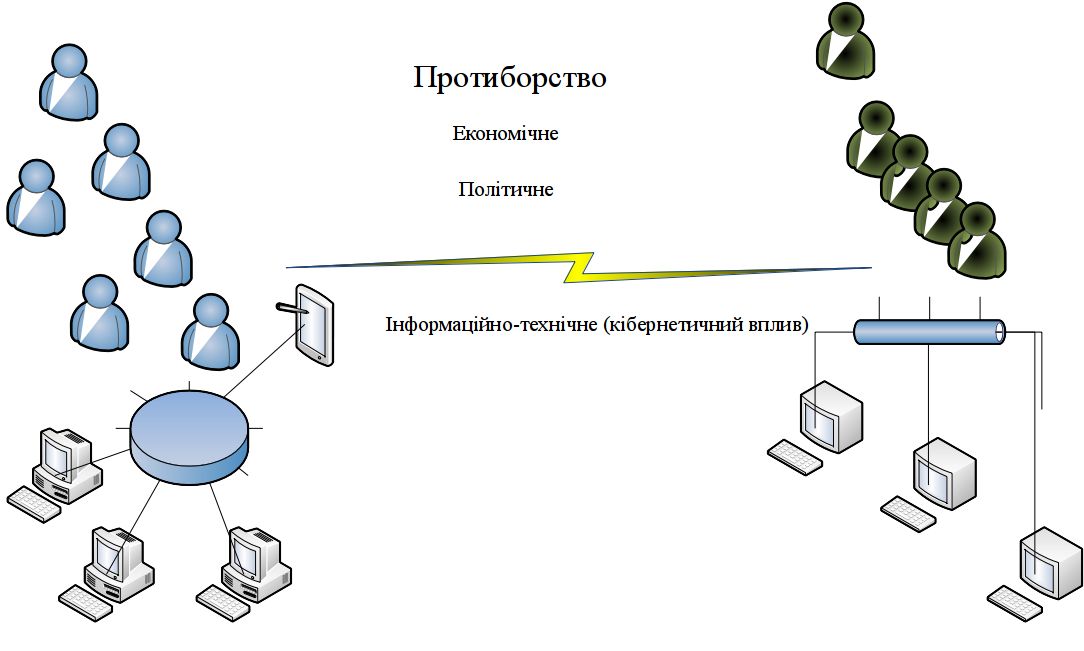
\includegraphics[width=15cm]{pic_cyber1.png}
    \caption{схема кібернетичного впливу}
    \label{fig:cyber_attack}
\end{figure}

Одним із підходів до підготовки військових фахівців, які здатні підтримувати безпеку у кібернетичному просторі – комунікаційному просторі, який охоплює комп’ютерні мережі та електронні пристрої, що використовуються для збереження, обробки та обміну інформацією є підготовка фахівців, що починається з формуванння бази до кваліфікаційного рівня бакалавр, а саме проходження циклів підготовки.
Підготовка фахівців з інформаційної безпеки (Рис \,\ref{fig:cyber_attack})

починається у циклі професійної і практичної підготовки, де на вивчаємих дисциплінах майбутніми фахівцями вивчаються матеріали, для формування загальних знань з комп’ютерних наук, вивчаються мови програмування, технології створення програмних продуктів, архітектура комп’ютерних та операційних  систем. Але щоб стати фахівцем, потрібна додаткова підготовка яка отримується після захисту кваліфікаційної роботи, майбутні фахівці розподіляються за спеціалізаціями підготовки, фахівці формуються відповідно до спеціалізації.

На етапі підготовки згідно спеціалізації вивчаються такі дисципліни як:
\begin{itemize}
\itemЕксплуатація та бойове застосування програмних засобів інформаційної боротьби в комп’ютеризованих системах та мережах спеціального призначення;
\itemМетодологічні основи інформаційної боротьби в комп’ютеризованих системах та мережах спеціального призначення;
\itemТехнології побудови програмних засобів інформаційної боротьби та ін.
\end{itemize}


\begin{figure}[h]
    \centering
    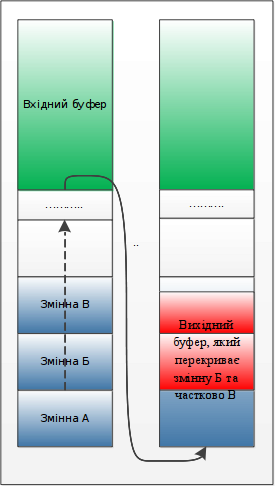
\includegraphics[height=10cm]{pic_bo_0.png}
    \caption{схема переповнення буфера}
    \label{fig:buffer_overflow}
\end{figure}

На етапі підготовки згідно спеціалізації потрібно приділяти багато уваги практичній підготовці та інтерактивному навчанню. Для цьго пропонується підхід до створення тренувального середовища із завідомо впровадженими вразливостями для нав’язування тестових впливів. Це середовище може слугувати матеріалом для вивчення вищеназваних дисциплін, як для відпрацювання технології побудови програмних засобів інформаційної боротьби,  для відпрацювання методології впливу на програмні продукти, а також використання програм для сканування вразливостей.

Необхідно виділити найбільш небезпечні вразливості для створення такої системи, кожна з уразливостей потребує детального вивчення, це окрема спеціалізація,  яка рамках підготовки фахівця з інформаційної безпеки потребує глибокого дослідження.
Досить розповсюдженим видом комп'ютерних атак на інформаційні системи є атака на переповнення буфера.
Переповнення буфера було та залишається дуже важливою проблемою в аспекті безпеки програмного забезпечення. Переповнення буфера (англ. buffer overflow або англ. buffer overrun), це явище, при якому програма, під час запису даних в буфер, перезаписує дані за межами буфера.
(Рис.\,\ref{fig:buffer_overflow})


Це може викликати несподівану поведінку, включно з помилками доступу до даних, невірними результатами, збоєм програми або дірою в системі безпеці.
Переповнення буфера може бути викликане недостатньою перевіркою вхідних даних. Воно є базою для багатьох уразливостей в програмних продуктах і може бути злонамірено використане.

Проблема переповнення буфера з роками тільки ускладнювалася, з'являлися типи атак, в результаті були розроблені принципово нові атаки на переповнення буфера.
Оскільки значна частка програмного забезпечення створюється на мові C/C++, в якій немає вбудованих засобів обробки рядків - а саме контролю розподілу пам’яті, тому вони використовують небезпечний програмний код, що не перевіряє довжину буфера, у який записуються зовнішні дані, отримані ззовні, внаслідок чого можливість перезапису інших даних програми, включаючи код, що дозволяє змінити виконання програми, незалежно коду. Атаки, в основному, здійснюються на програмні застосування, виконуються в привілейованому режимі, що дозволяє підняти рівень привілеїв для виконання шкідливого коду.
Зробивши аналіз найбільш поширених прийомів техніки переповнення буферу можна зробити висновок що фахівцям в даній предметній області необхідно мати глибокі знання в таких дисциплінах як:
\begin{itemize}
\itemопераційні системи(знання архітектури ОС Linux/Unix-like/WinX);
\itemсистемне, мережеве програмування (низькорівневе);
\itemтеорії побудови компіляторів / інтерпретаторів – теорія кінцевих автоматів;
\itemпрактичні навички використання засобів відлагодження та дослідження програмних продуктів;
\end{itemize}

\upshape{Типові ситуації використання переповнення буфера.}

Техніки використання уразливості через переповнення буфера залежать від архітектури, операційної системи і ділянки пам'яті 
%(рис.1.5.)
.
Існують наступні види переповнення буфера:
\begin{itemize}
\itemпереповнення у стекові (stack smashing - зрив стеку), який полягає у перезаписі адреси повернення з вразливої функції, що призводить до виконання коду(існуючого або підготовленого зловмисником) за адресом, вказаним атакуючим;
\itemпереповнення в сегментах даних та динамічних областях (DATA, BSS, HEAP overflow), яке являє собою корекцію набору даних, керуючих алгоритмом програми, а також вказівників на функції, класи та управління. 
\end{itemize}


Технічно освідомлений і злонамірений користувач може використати стекове переповнення буфера так:
\begin{enumerate}
\itemДля перезапису локальної змінної, змінивши тим самим перебіг програми на більш вигідний для нападника.
\itemДля перезапису адреси повернення в стековому кадрі. Коли буде виконане повернення з функції, виконання програми відновиться за адресою, вказаною нападником (зазвичай це адреса буфера поля вводу). Такий спосіб найбільш розповсюджений в архітектурах, де стек росте донизу (наприклад в архітектурі x86).
\itemДля перезаписів вказівника на функцію, або обробника винятків, що будуть виконані згодом. 
\end{enumerate}

Два основних типи даних, які дозволяють здійснити переповнення буфера в цих мовах — рядки і масиви. Таким чином, використання бібліотек для рядків і спискових структур даних, які були розроблені для запобігання і/або виявлення переповнень буфера, дозволить уникнути уразливостей.
Шелкод (Корисне навантаження) ( англ. {\it shellcode}, код запуску оболонки) - це двійковий виконуваний код, який зазвичай передає управління командному процесору,  наприклад `{\it / bin / sh}'  {\it Unix Shell}, {\it command.com} в {\it MS-DOS} і {\it cmd.exe} в операційних системах {\it Microsoft Windows}.  Шелкод може бути використаний як корисне навантаження експлойту, що забезпечує зловмисникові доступ до командного інтерпретатра (англ.{\it shell}) в комп'ютерній системі.

При експлуатації віддаленої уразливості шелкод може відкривати заздалегідь заданий порт {\it TCP} уразливого комп'ютера, через який буде здійснюватися подальший доступ до командної оболонці, такий код називається прив'язує до порту ( англ. {\it port binding shellcode}).  Якщо шелкод здійснює підключення до порту комп'ютера атакуючого, що проводиться з метою обходу брандмауера або {\it NAT}, то такий код називається зворотної оболонкою ( англ. {\it reverse shell shellcode}).
Шелкод зазвичай впроваджується в пам'ять експлуатованої програми, після чого на нього передається управління шляхом переповнення стека, або при переповненні буфера в купі, або використовуючи атаки форматної рядка.  Передача управління шелкоду здійснюється перезаписом адреси повернення в стеку адресою впровадженого шелкоду, перезаписом адрес викликаються функцій або зміною обробників переривань.  Результатом цього є виконання шелкоду, який відкриває командний рядок для використання зломщиком.

Розрізняють два типи шелкоду :
\begin{itemize}
\itemлокальний (впровадження та виконання можливе тільки за безпосереднього доступу зловмисника до КС)
\itemвіддалений (атака з віддаленої машини). 
\end{itemize}

Локальний шелкод використовується зловмисником, коли він обмежений в правах комп’ютерної системи, але може використати вразливість в програмному забезпеченні даної системи з підняттям привілеїв до того рівня що і цільовий процес.

Віддалений шелкод використовується хакерами для захоплення контролю над процесом на віддаленій машині в локальній мережі чи в інтернеті. У разі успішного його виконання, хакер матиме можливість отримати доступ над машиною по мережі. Віддалені шелкоди переважно використовують  {\it TCP/IP}-зєднання для забезпечення атакуючого доступом до командної оболонки. Такий шелкод може бути класифікований по тому, як він встановлює з’єднання.: якщо код може встановити з’єднання, його називають ``{\it reverse shell}'' або “{\it connect-back shellcode}”
%(рис.1.6.)
, так як він з’єднується з машиною атакуючого. З іншого боку, якщо зловмисник потребує встановити з’єднання, то такий шелкод називають “{\it  bindshell}”, так як він відкриває і прослуховує порт, по якому зловмисник може під’єднатися і отримати контроль над системою. Є третій тип, менш використовуваний, має назву “{\it socket-reuse shellcode}”. Цей тип шелкоду іноді використовується, коли експлойт встановлює з’єднання з вразливим процесом, який до його запуску не закрив з’єднання. Тому він може використати з’єднання для комунікації з хакером для віддаленого управління системою. Цей тип шелкоду є складним в реалізації так як він повинен виконати пошук вразливого процесу, який має відкрите з’єднання.

\pagebreak

\section{Дослідження початкового тексту як метод виявлення потенційно-небезпечних дефектів програм.}
\label{1section:id3}
На сьогоднішній час існує низка засобів для аналізу програм як у вигляді вихідних текстів так і у двійковому коді.
Для виявлення вразливостей захисту в програмах застосовують такі інструментальні засоби:
\begin{itemize}
\itemдинамічні відлагоджувачі. Інструменти, які дозволяють виробляти налагодження програми в процесі її виконання;
\itemстатичні аналізатори (статичні відлагоджувачі).
\end{itemize}

Інструменти, які використовують інформацію, накопичену в ході статичного аналізу досліджуваної програми.

Статичні аналізатори вказують на ті місця в програмі, в яких можливо знаходиться помилка. Ці підозрілі фрагменти коду можуть, як містити помилку, так і не нести ніякої небезпеки для виконання програми. Наявність вихідних кодів програми істотно спрощує пошук вразливостей.
Розглянемо декілька інструментів для аналізу вихідних текстів досліджуваних програм:

Інструмент {\it BOON}, який на основі глибокого семантичного аналізу автоматизує процес сканування вихідних текстів на Сі в пошуках уразливих місць, здатних призводити до переповнення буферу. Він виявляє можливі дефекти, припускаючи, що деякі значення є частиною неявного типу з конкретним розміром буфера.

{\it CQual} - інструмент аналізу для виявлення помилок в Сі-програмах. Програма розширює мову Сі додатковими обумовленими користувачем специфікаторами типу. Програміст коментує свою програму з відповідними специфікаторами, і {\it cqual} перевіряє помилки. Неправильні анотації вказують на потенційні помилки. {\it Сqual} може використовуватися, щоб виявити потенційну уразливість форматною рядка.

{\it MOPS} - інструмент для пошуку вразливостей в захисті в програмах на Сі. Його призначення: динамічне коректування, що забезпечує відповідність програми на Сі статичної моделі. {\it MOPS} використовує модель аудиту програмного забезпечення, яка покликана допомогти з'ясувати, чи відповідає програма набору правил, визначеному для створення безпечних програм.

{\it ITS4}. Простий інструмент, який статично переглядає вихідний Сі / Сі++ - код для виявлення потенційних вразливостей захисту. Він зазначає виклики потенційно небезпечних функцій, таких, наприклад, як {\it strcpy / memcpy}, і виконує поверхневий семантичний аналіз, намагаючись оцінити, наскільки небезпечний такий код, а так само дає поради щодо його поліпшення.

{\it RATS}. Утиліта {\it RATS (Rough Auditing Tool for Security)} обробляє код, написаний на Сі / Сі++, а також може обробити ще і скрипти на {\it Perl, PHP і Python. RATS} переглядає вихідний текст, знаходячи потенційно небезпечні звернення до функцій. Мета цього інструменту - не остаточно знайти помилки, а забезпечити обгрунтовані висновки, спираючись на які фахівець зможе вручну виконувати перевірку коду.{\it RATS} використовує поєднання перевірок надійності захисту від семантичних перевірок в {\it ITS4} до глибокого семантичного аналізу в пошуках дефектів, здатних привести до переповнення буфера, отриманих з {\it MOPS}.

{\it Flawfinder}. Як і {\it RATS}, це статичний сканер вихідних текстів програм, написаних на {\it С/С++}. Виконує пошук функцій, які найчастіше використовуються некоректно, присвоює їм коефіцієнти ризику (спираючись на таку інформацію, як передані параметри) і складає список потенційно вразливих місць, впорядковуючи їх за ступенем ризику.

Всі ці інструменти схожі і використовують тільки лексичний і найпростіший синтаксичний аналіз. Тому результати, видані цими програмами, можуть містити до 100\% помилкових повідомлень.

{\it Bunch} - засіб аналізу та візуалізації програм на Сі, яке будує граф залежностей, що допомагає аудитору розібратися в модульній структурі досліджуваної програми.

{\it Frama-C} - відкритий, інтегрований набір інструментів для аналізу вихідного коду на мові Сі. Набір включає {\it ACSL (ANSI / ISO C Specification Language)} - спеціальна мова, що дозволяє детально описувати специфікації функцій Сі, наприклад, вказати діапазон допустимих вхідних значень функції і діапазон нормальних вихідних значень.
\begin{quote}

Цей інструментарій допомагає виробляти такі дії:
\end{quote}
\begin{itemize}
\item {} 
здійснювати формальну перевірку коду;

\item {} 
шукати потенційні помилки виконання;

\item {} 
провести аудит або рецензування коду;

\item {} 
проводити реверс-інжиніринг коду для поліпшення розуміння структури програмного коду;

\item {} 
генерувати формальну документацію.

\end{itemize}

Також при відсутності вихідного тексту для аналізу програмного коду можна використовувати динамічні відлагоджувачі, які також можуть допомогти виявити помилки в коді, які допущені компілятором.
Найпоширенішими відлагоджувачами на даний момент є {\it SoftIce, OllyDebug, IDA Pro, GDB:}

{\it SoftIce} – всім відомий відлагоджувальник для ОС сімейства {\it Windows}, який працює в режимі ядра, що дозволяє відлагоджувати драйвера та різного роду сервіси що працюють в привілейованому режимі процесора. Працює в обхід {\it MS Debugging API}, що дуже ускладнює реалізацію захисту від відлагодження. {\it SoftICE}  був спочатку розроблений компанією {\it NuMega}, яка включала його в пакет програм для швидкої розробки високопродуктивних драйверів під назвою {\it Driver Studio}, який пізніше був придбаний {\it Compuware}.

{\it OllyDebug} – це 32-бітний відлагоджувальник працюючий в непривілейованому режимі процесора. Він має достатньо зручний інтерфейс та корисні функції які значно полегшують процес від лагодження.  В {\it OllyDBG} вбудований спеціальний аналізатор, який розпізнає і візуально позначає процедури, цикли, константи і рядки, звернення до функцій {\it API}, параметри цих функцій і т.п.

{\it IDA Pro} – це одночасно інтерактивний дизасемблер і відлагоджувальник. Він дозволяє отримати асемблерний текс, який може бути застосований для аналізу роботи програми. Варто зазначити, що вбудований відлагоджувальник доволі примітивний, працює через {\it MS Debugging API (в NT)} і через бібліотеку ptrace (в {\it UNIX}), що робить його легкорозпізнаємим для захисних механізмів. Сильною стороною цього продукту є саме дизасемблер, який на сьогодні генерує якісний вихідний текс. Окрім цього існує велика кількість плагінів під даний програмний продукт, що значно розширює його можливості. Також можливе написання плагінів на скрипкових мовах – є підтримка {\it Ruby, Python}.

{\it GDB - GNU Debugger} – основний відлагоджувальник під {\it UNIX}, орієнтований на зовсім інший тип мислення, аніж всі вищеперераховані відлагоджувальники. Це не просто інтерактивний відлагоджувальник – це модуль управління виконанням програм з гнучким і потужним інтерфейсом. Негативною стороною даного відлагоджувальника є відсутність аналізу захисних механізмів програм, тому у разі їх присутності в коді – процес відлагоджування стає неможливим.

Дані програмні засоби добре справляються з заявленими ними завданнями, але враховуючи тенденції теперішніх технологій та стрімкий ріст розмірів як вихідних текстів програм так і їх двійкових образів, завдання швидкого аналізу дещо ускладюється насамперед тим, що результати аналізу містять надмірну кількість інформації, яку такок потрібно аналізувати. Тому виникає потреба в більш загальному аналізі характеристик коду, який дасть якісну оцінку окремих частин досліджуванної програми, що дозволить диференціювати задачу аналізу та правильно його організувати.

Завдання оцінки інтегрованих властивостей програм в певній мірі вирішують так звані метрики коду. 

Метрика якості програм - система вимірювань якості програм . Ці виміри можуть проводитися на рівні критеріїв якості програм або на рівні окремих характеристик якості. У першому випадку система вимірювань дозволяє безпосередньо порівнювати програми за якістю. При цьому самі виміри не можуть бути проведені без суб'єктивних оцінок властивостей програм. У другому випадку вимірювання характеристик можна виконати об'єктивно і достовірно, але оцінка якості ПЗ в цілому буде пов'язана з суб'єктивною інтерпретацією одержуваних оцінок.

\pagebreak

\section*{Висновки}
\addcontentsline{toc}{section}{Висновки}
Отже, в зрізі теперішніх тенденцій інформаційних технологій  - а саме стрімкого росту розмірів як вихідних текстів програм так і їх двійкових образів виникає потреба в більш загальному аналізі характеристик коду, який дасть якісну оцінку окремих частин досліджуванної програми, що дозволить диференціювати задачу аналізу та правильно його організувати.
